\section{Task 1: Model for Tourism Industry in Juneau}

\subsection{Introduction}


In this section we need to select factors to quantify and track the tourism industry in Juneau. 
It is impossible and unnecessary to consider all the factors that may affect the 
tourism industry, only those that are relevant to the problem need to be considered.
Drawing on the idea of the divide-and-conquer algorithm, we first divide the factors 
into three categories: economy, environment and society(aka hidden causes). 
The untimate goal is listed below:


\begin{equation}
    \mathcal{F}=(\alpha \cdot \text { Economy }-\beta \cdot \text { Environment }) \cdot \text { Hidden Causes }
\end{equation}

where $\alpha$ and $\beta$ are the weights of the economy and environment, denoting the importance we attach to each category.
Economy means the income generated by the tourism industry, environment means the environmental cost of the tourism industry, and 
society is an indicator that quantifies the satisfaction of the local residents towards the tourism industry.

Our goal is to maximize the final output $\mathcal{F}$. Intuitively, it 
is equivalent to maximizing economy income, minimizing the environmental 
impact and elevating the final scores of hidden causes.

Each category is further divided into several minor factors such as local population, 
number of tourists to extrapolate a mathematical model fitting the circumstances in Juneau,
which will be discussed in the following sections.





\subsection{Economy}

In this section we consider the actions that will contribute to the income of the tourism industry in Juneau, which are
tourists' consumption, tax income and fines.

\subsubsection{Tourists' Consumption}

We first calculate the average consumption of tourists in Juneau per day. Since there is no existing official data available, 
we can infer it by other means. According to [source], avearge tax income from tourists in Juneau is 27.7 million dollars in 2018
with a tax rate of 12\%. We can use this information to estimate the average consumption of tourists in Juneau per day according to 
the following equation.

\begin{equation}
    \text{Average Consumption} = \frac{\text{Tax Income}}{\text{Tax Rate} \times \text{Number of Tourists}}
\end{equation}

The number of tourists can be found in Table 2. The average consumption of 
tourists in Juneau per day is calculated as follows:

\begin{equation}
    \text{Average Consumption} = \frac{27.7 \times 10^6}{0.12 \times 1151 \times 10^3} \approx 200.55
\end{equation}

Therefore the function of tourists' consumption regarding the number of tourists is:


\begin{equation}
    \text{Tourists' Consumption} = 200.55 N
\end{equation}

Given that an average of 3 days are spent by each visitor to Juneau, 
the total consumption of tourists should multiply by another 3.

\subsubsection{Tax Income}

According to the official website of Juneau, the tax rate of the tourism industry is 12\%.
The tax income can be calculated as follows:

\begin{equation}
    \text{Tax Income} = 0.12 \times \text{Tourists' Consumption} \approx 24 N
\end{equation}

We should also consider the case when the tax rate is not fixed to propose suggestions to the
government on how to adjust the tax rate to maximize the income of the tourism industry. We
use the data calculated as above as the base case and assume that the tex rate $\eta$ is associated with the number of tourists.

The actual visitors $N$ is calculated as follows:


\begin{equation}
    N= N_0 \cdot f(\eta)
\end{equation}

Intuitively, $\eta$ should be negatively correlated with the number of tourists. When $eta$ is 
set to 0, we assume that the number of tourists will be $1.5N_0$, and when $\eta$ is set to 1, the number of tourists will be 0.
Specifically, when $\eta$ is set to the current tax rate 0.12, the number of tourists will be $N_0$. 
Also, $f(\eta)$ should be monotonically decreasing and fall steeply in the range of $[0,0.12]$ and $[0.85,1]$, 
Using the above data
we propose a model that fits the relationship between the tax rate and the number of tourists as follows:

\begin{equation}
    f(\eta) = -5.5 \eta^3 + 9.1903 \eta^2 - 5.1903 \eta + 1.5, \quad 0 \leq \eta \leq 1
\end{equation}

Therefore the tax income can be calculated as follows:

\begin{equation}
    \text{Tax Income} = 200.55N \cdot f(\eta), \quad 0 \leq \eta \leq 1
\end{equation}

\subsubsection{Fines}

As there is no official data available, we assume that the 
fine rate is negatively correlated with the amount of fines 
and follows an exponential distribution $f(x) = \lambda \cdot e^{-\lambda x}$. We also assume that 
fined rate falls to 5\% when the amount of fines climbs to 15 dollars, that is:

\begin{equation}
    \int_0^{15} \lambda \cdot e^{-\lambda x} d x=1-95 \% \Rightarrow \lambda \approx 0.2
\end{equation}

Therefore the total amount of fines can be calculated as follows:

\begin{equation}
    \text { Fines }=N Q \cdot\left(1-\int_0^Q 0.2 \cdot e^{-0.2 x} d x\right)=N Q \cdot e^{-0.2 Q}
\end{equation}




\subsection{Environment}

% According to the official website of Juneau, its tourism industry is 
% mainly comprised of glacier tours, whale watching, rainforest tours and others.
% We assume each of these activities accounts for a certain percentage of the total environmental impact,
% denoted as $v_1$, $v_2$, $v_3$ and $v_4$ respectively. Due to the receding of glaciers,
% our goal is to lower the percentage of glacier tours and increase the percentage of other activities.

In this section we propose a new model $KAYA_{tourism}$ derived 
from the KAYA model to quantify the environmental impact of the tourism industry in Juneau.

\subsubsection{KAYA Model}

The original KAYA model is a mathematical model that 
describes the relationship between the total 
amount of CO2 emissions and the four factors 
that affect it: population, GDP per capita, energy intensity and carbon intensity.
 The KAYA model is expressed as follows:

\begin{equation}
    \text { CO2 Emissions }=P \times GDP \times E I \times C I
\end{equation}

where $P$ denotes the population, $GDP$ denotes the GDP per capita, 
$EI$ denotes the energy intensity and $CI$ denotes the carbon intensity.
This model falls short when only considering the environmental impact of the tourism industry.
Based on the data we collect and the goal of our project, we propose a new model $KAYA_{tourism}$.


\subsubsection{$KAYA_{Tourism}$ Model}

The $KAYA_{Tourism}$ model is expressed as follows:

\begin{equation}
    CO_{2\_Tourism}=G \times CG_{Tourism}
\end{equation}

where $G$ denotes the gross income of the tourism industry and $CG = EI \times CI$. To calculate 
the emission of $CO_2$ in the tourism industry, we first looked up the data of the Juneau's carbon emission and
GDP across the country and calculated the $CG_{All}$ across the country. $CG_{Tourism}$ can 
be calculated as $CG_{Tourism} = CG_{All} \times Ratio $  where $Ratio$ is the 
ratio tourism accounts for across all industries. The income of the tourism industry in Juneau 
has been calculatd in the previous section, and the $CO_{2\_Tourism}$ can thus be estimated.
It should be noted that $G$ and $CG_{Tourism}$ are both linear functions of the number of tourists $N$,
therefore when fitting and regressing $CO_{2\_Tourism}$ quadratic regression should be used.

Alongside the historical data, future predictions are also conducted using the \textit{SARIMAX} model.
The results are listed below.

\begin{figure}[H]
    \centering
    \begin{minipage}{0.32\textwidth}
        \centering
        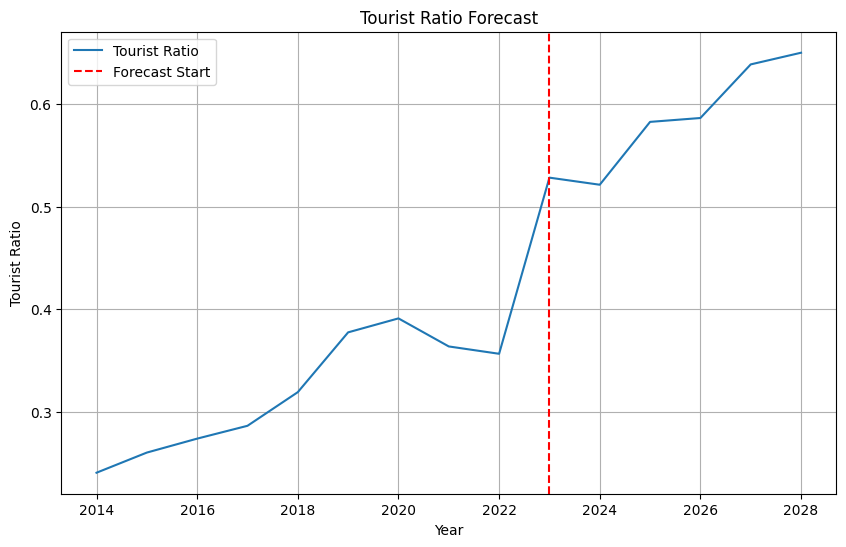
\includegraphics[width=\textwidth]{Ratio.png}
        % \caption{Caption 1}
    \end{minipage}
    \begin{minipage}{0.32\textwidth}
        \centering
        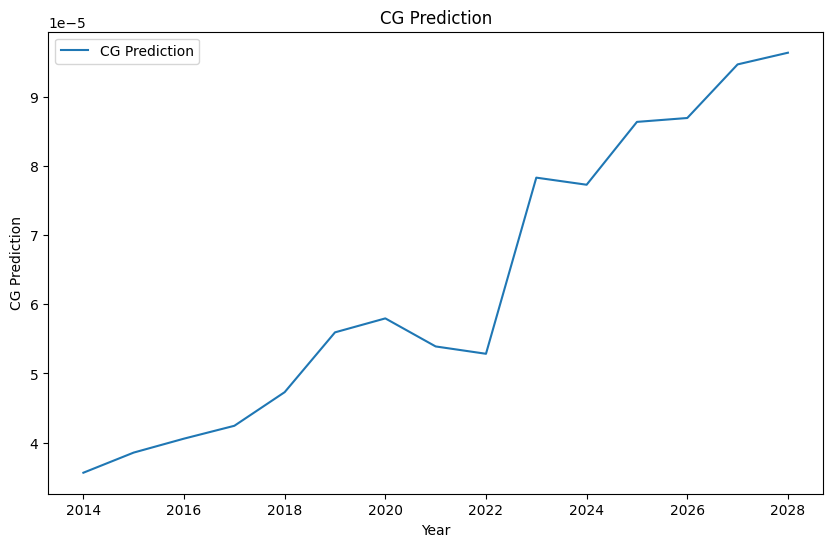
\includegraphics[width=\textwidth]{CG_pred.png}
        % \caption{Caption 2}
    \end{minipage}
    \begin{minipage}{0.32\textwidth}
        \centering
        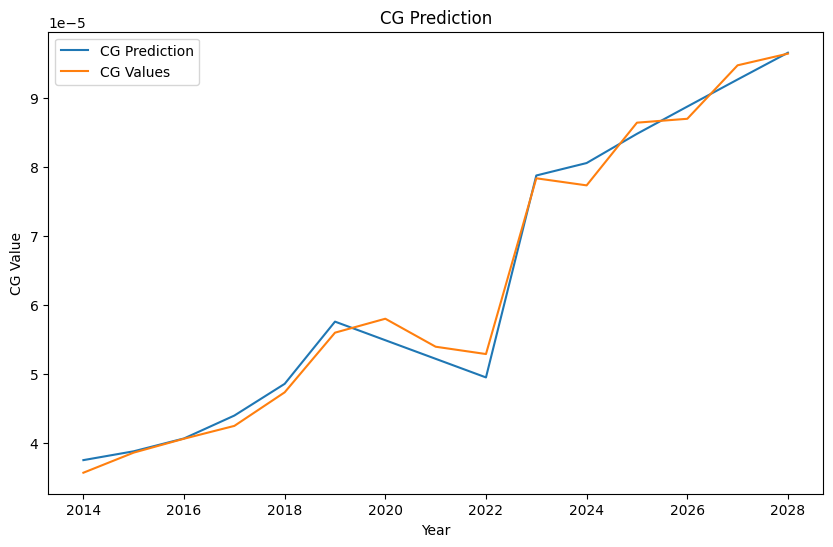
\includegraphics[width=\textwidth]{CG_pred2.png}
        % \caption{Caption 3}
    \end{minipage}
\end{figure}

\begin{figure}[H]
    \centering
    \begin{minipage}{0.32\textwidth}
        \centering
        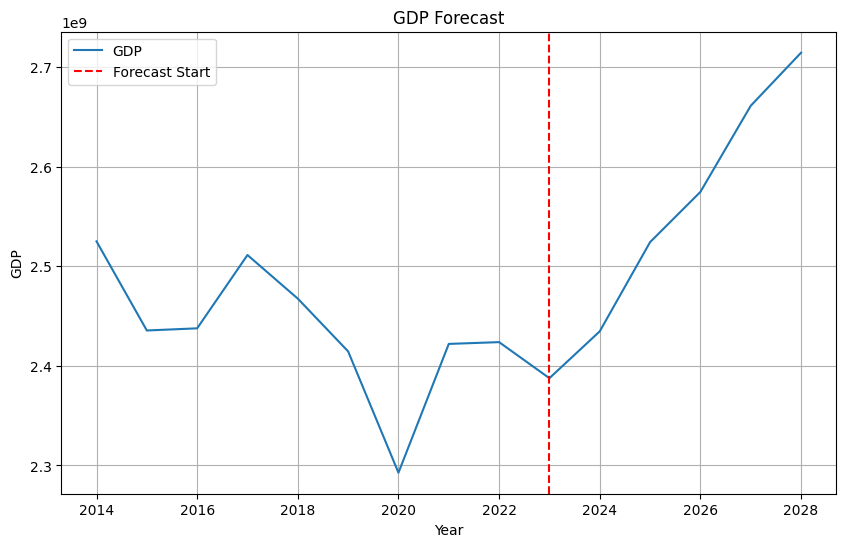
\includegraphics[width=\textwidth]{GDP.png}
        % \caption{Caption 4}
    \end{minipage}
    \begin{minipage}{0.32\textwidth}
        \centering
        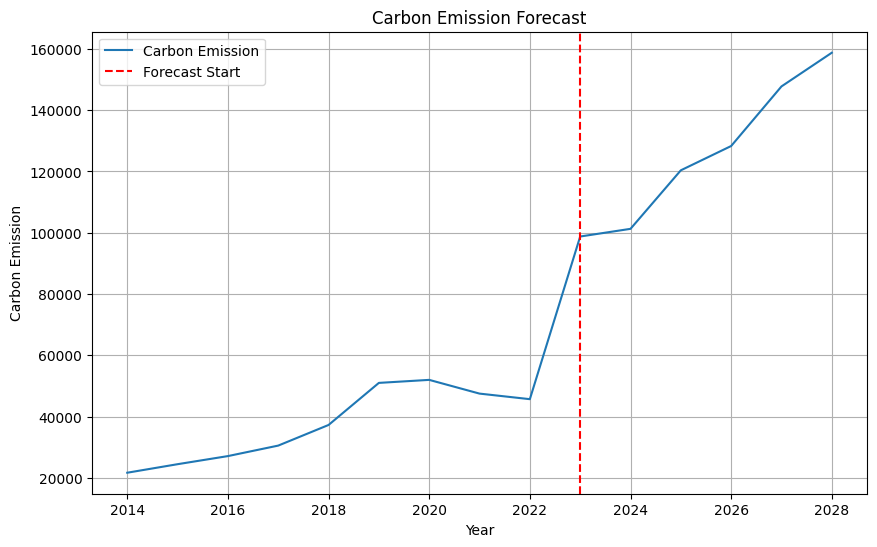
\includegraphics[width=\textwidth]{Emission.png}
        % \caption{Caption 5}
    \end{minipage}
    \begin{minipage}{0.32\textwidth}
        \centering
        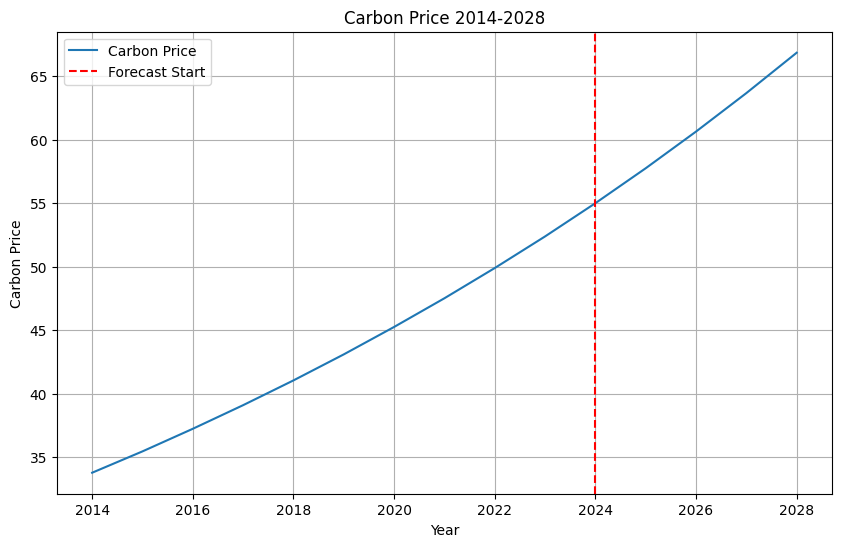
\includegraphics[width=\textwidth]{Price.png}
        % \caption{Caption 6}
    \end{minipage}
\end{figure}

\begin{figure}[H]
    \centering
    \begin{minipage}{0.32\textwidth}
        \centering
        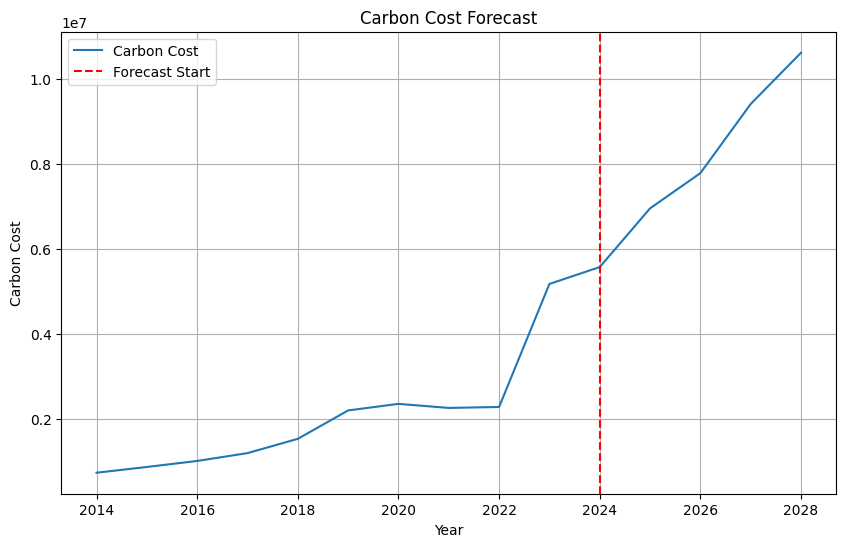
\includegraphics[width=\textwidth]{Cost.png}
        % \caption{Caption 7}
    \end{minipage}
    \begin{minipage}{0.32\textwidth}
        \centering
        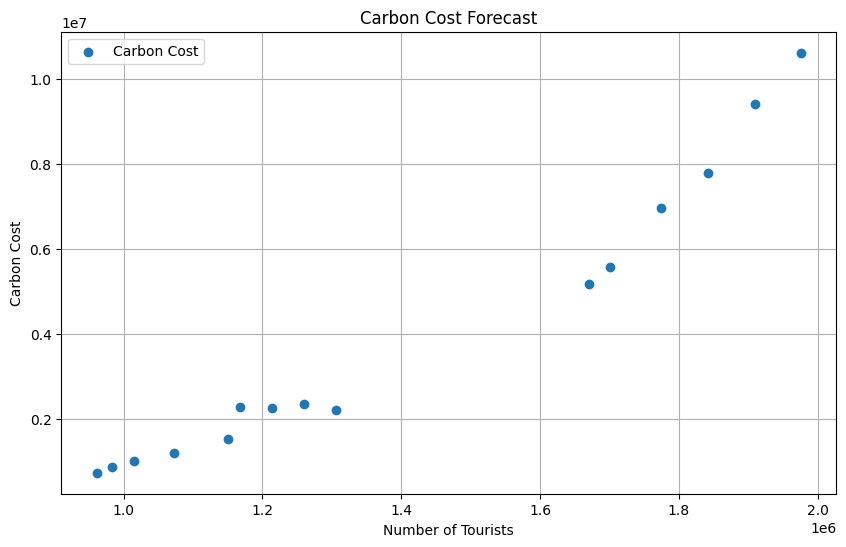
\includegraphics[width=\textwidth]{Carbon_pred1.png}
        % \caption{Caption 8}
    \end{minipage}
    \begin{minipage}{0.33\textwidth}
        \centering
        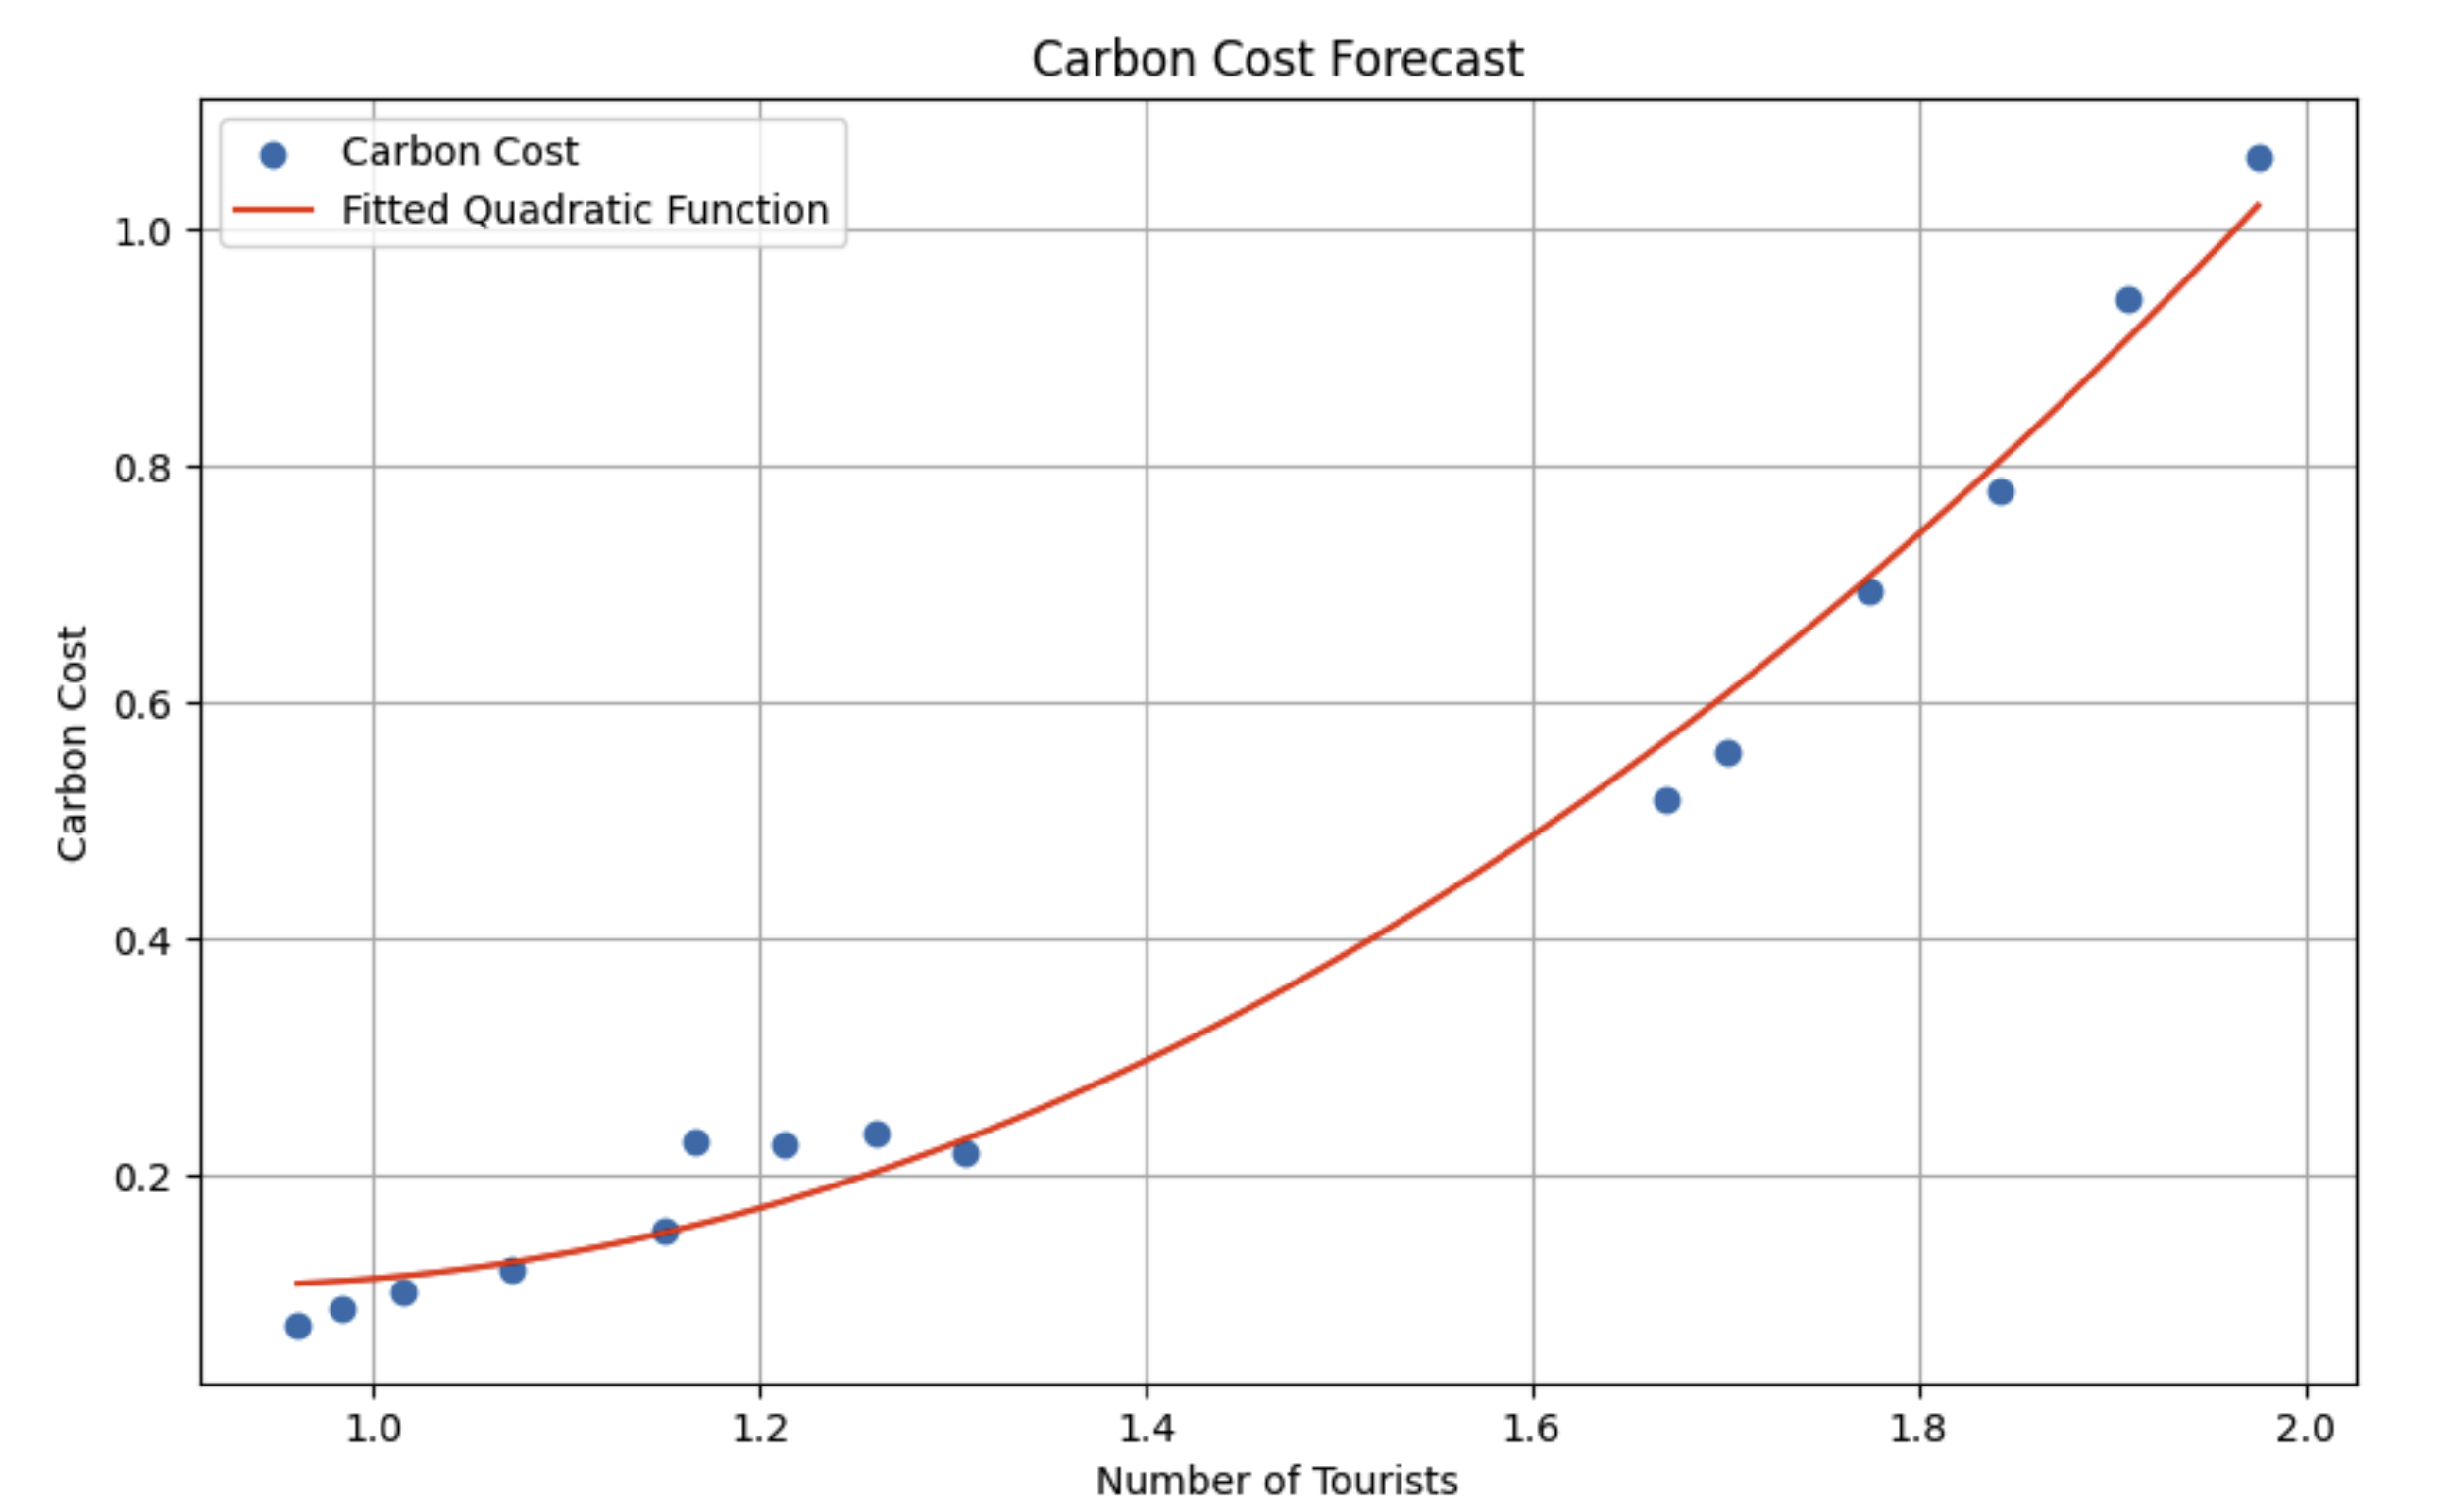
\includegraphics[width=\textwidth]{Carbon_pred2.png}
        % \caption{Caption 9}
    \end{minipage}
\end{figure}

From subplot 9 we can see that a quadratic regression 
fits the data well with an $R^2$ value of over 0.99.
The fitting function yields the following results:

\begin{equation}
    CO_{2\_Tourism} = 0.815 \times \frac{N^2}{10^5} - 14.95N+7924000
\end{equation}



\subsection{Hidden Causes}

Societal factors such as infrastructure, price of housing products, and the mental
loss due to the overcrowding and rowdy tourists all account for the hidden costs of the tourism industry.

The result yields:

\begin{equation}
    \text {Score}=5.011\times 10^{-9} N -0.002 \times N_{Local}+69.93
\end{equation}


\subsection{Summary}



Summing up all the three categories, we can get the final output of the model:

\begin{equation}
    \begin{aligned}
    &\left\{\begin{array}{l}
    F=(\alpha \cdot \text { Economy }-\beta \cdot \text { Environment }) \cdot \text { Society } \\[10pt]
    \text { Economy }=200.55 N \cdot(f(\eta)+1) \cdot (\eta+1)+NQ\cdot e^{-0.2 Q} \\[10pt]
    \text { Environment }=0.815 \cdot \frac{N^2}{10^5}-14.95 N+7924000 \\[10pt]
    \text { Society }=5.011\times 10^{-9} N -0.002 \times N_{Local}+69.93 \\[10pt]
    f(\eta)=-5.5 \eta^3+9.1903 \eta^2-5.1903 \eta+1.5, \quad 0 \leq \eta \leq 1
    \end{array}\right.
    \end{aligned}
\end{equation}

where $N,Q,\eta$ are independent variables, $\alpha$, $\beta$ 
and are parameters that can be adjusted accordingly, 
$N_{Local}$ is the local population of Juneau assumed fixed.
Our goal is to find the optimal value of $N,Q,\eta$ that maximizes the output $\mathcal{F}$.

\subsection{Sensitivity Analysis}

To evaluate the robustness of our model, we conduct a sensitivity analysis.

\subsubsection{Principal Component Analysis}

Principal Component Analysis (PCA) is a statistical method that
extracts the most important information from a dataset and
presents it as a set of new variables called principal components.
The first principal component accounts for the largest variance in the data,
the second principal component accounts for the second largest variance, and so on.
The results of the PCA are shown below.


\subsubsection{Analysis of the Results}

It can be seen that the government should adjust the tax rate to 0.12 to 
maximize the income of the tourism industry. The number of tourists should be
around 1151, and the fine rate should be set to 0.15 to maximize the income of the tourism industry.